\chapter{Caching}

\section{Funzionamento di Base di una Cache}

La memoria principale è sempre stata più lenta di una CPU, questo gap si è ampliato ulteriolmente nel tempo.

\begin{figure}[!h]
    \centering
    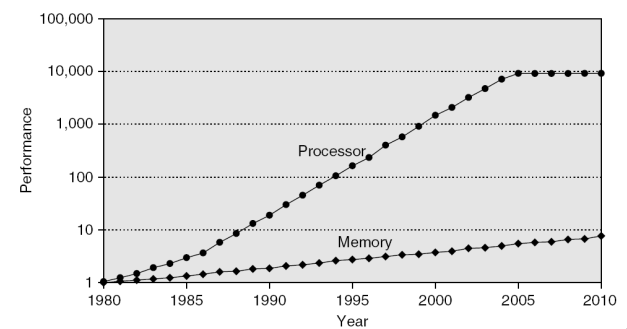
\includegraphics[scale=0.7]{03-Cache/PvsM.png}
    \caption{Andamento nel tempo.}
\end{figure}

\nt{Inoltre la situazione peggiora ancora se si considerano anche i processori multi-core.}

\clm{}{}{
  \begin{itemize}
    \item Il termine SRAM (Static RAM) indica la tecnologia di base con cui sono costruite le RAM usate nei vari livelli di cache del processore. 
    \item Le SRAM usano un circuito di transistor che devono essere sempre alimentati. 
    \item Le DRAM usano un condensatore la cui carica indica se un bit vale 0 o 1. Ogni pochi millisecondi viene fatto un refresh.
    \item Le SRAM sono più veloci, ma consumano di più, sono più complesse e consumano di più.
    \item La cache L1 è ottimizzata rispetto alla velocità di accesso, mentre L2 e L3 rispetto alla capienza di memorizzazione. 
  \end{itemize}
}

\paragraph{Il concetto di caching:}

\begin{itemize}
  \item I registri fanno da cache per la cache hardware. 
  \item La cache hardware fa da cache per la RAM. 
  \item La RAM fa da cache per l'Hard disk (memoria virtuale). 
  \item L'hard disk fa da cache per supporti magnetici più lenti.
\end{itemize}

\dfn{Gerarchi di cache}{
  \begin{itemize}
    \item L1: due cache, una per la data memory  l'altra per la instruction memory. 
    \item L2 e L3 (non in tutti).
  \end{itemize}
}

\begin{figure}[!h]
    \centering
    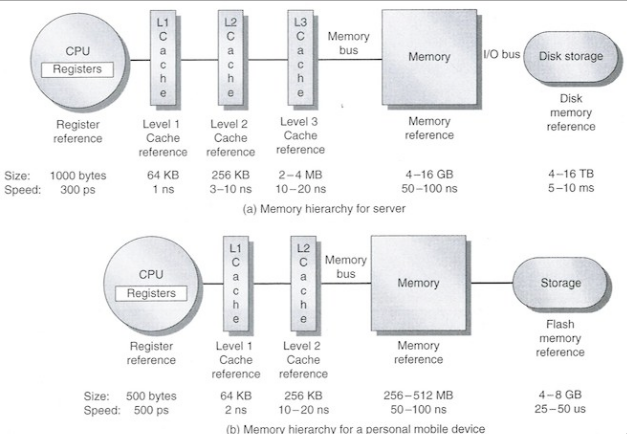
\includegraphics[scale=0.5]{03-Cache/gerarchia.png}
    \caption{Gerarchia di memorie.}
\end{figure}

\cor{Località Spaziale}{
  Area di memoria con indirizzi simili a quelli appena usati, saranno a loro volra usate nell'immediato futuro. 
}

\cor{Località Temporale}{
  Locazioni accedute di recente verranno di nuovo accedute nell'immediato futuro.
}

\dfn{Linee}{Per permettere l’interazione tra memoria cache e RAM, entrambe
sono suddivise in blocchi di dimensione fissa dette linee di cache e
linee di RAM rispettivamente.}

\clm{}{}{
  \begin{itemize}
    \item Ogni linea è identificata dal suo indirizzo in RAM. L'indirizzo in RAM del primo byte appartenente a quella linea.
    \item Il numero della linea dipende dagli m bit più significativi.
  \end{itemize}
}

\cor{Cache Hit}{
  Se viene indirizzata una word che si trova nella cache si ha un cache hit: tutto procede normalmente in quanto la cache è in grado di lavorare alla stessa velocità degli altri elementi del datapath.
}

\cor{Cache Miss}{
  Se viene indirizzata una word che non si trova nella cache si ha un cache miss: il dato viene prelevato dalla RAM e se necessario una linea della cache viene rimossa per fare spazio a quella mancante.
}

\cor{Penalità da fallimento}{Il tempo necessario a recuperare un dato in RAM quando si verifica un cache miss.}

\paragraph{La durata della penalità da fallimento è dovuta a:}

\begin{itemize}
  \item Inviare l'indirizzo della linea mancante alla RAM. 
  \item Accedere alla RAM per recuperare la linea. 
  \item Inviare alla cache la linea recuperata.
\end{itemize}

\subsection{Cache Direct-Mapped}

\dfn{Cache Direct-Mapped}{
Le cache Direct-Mapped (in italiano: a indirizzamento diretto)
sono il tipo di cache più semplice. Una cache Direct-Mapped è
formata da $2^k$ entry numerate consecutivamente.

Ogni entry memorizza 32 o 64 byte consecutivi e ha associate due informazioni:

\begin{itemize}
  \item Un \textit{bit di validità} che dice se quella entry contiene dell'informazione significativa. 
  \item Un campo \textit{TAG} che identifica univocamente la linea contenuta in quella entry della cache rispetto a tutte le linee della RAM.
\end{itemize}

}
 \nt{In una cache direct-mapped ogni linea della RAM viene memorizzata in una entry ben precisa della cache. Per stabilire in quale entry della cache cercare una linea che contiene il dato o l'istruzione indirizzati dalla CPU si usa l'operazione: (numero della linea in RAM) modulo (numero di entry nella cache).}

\begin{figure}[!h]
    \centering
    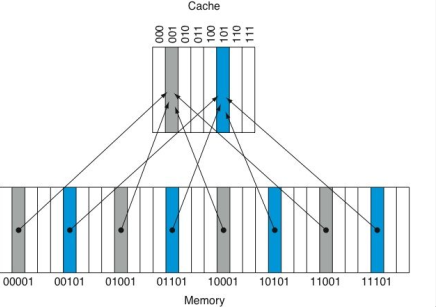
\includegraphics[scale=0.5]{03-Cache/Cache ad accesso diretto.png}
    \caption{Linee di cache.}
\end{figure}

\paragraph{I 32 bit di cui è composto l'indirizzo sono suddivisi in:}

\begin{itemize}
  \item \fancyglitter{TAG:} 16 bit più significativi dell’indirizzo generato dalla CPU,
usati per distinguere fra loro le linee di RAM che fanno capo alla
stessa entry in cache. 
\item \fancyglitter{CACHE ENTRY:} gli 11 bit che indicano in quale entry della
cache cercare la linea che contiene il dato/istruzione indirizzato. 
\item \fancyglitter{WORD:} i 3 bit con cui distinguiamo fra loro le 8 word contenute
in una linea da 32 byte. 
\item \fancyglitter{BYTE:} i 2 bit che possono servire a individuare i singoli byte di
cui è composta ciascuna word.
\end{itemize}

\nt{Le prestazioni di una cache dipendono, oltre che dal numero di linee di RAM che è in grado di memorizzare, anche dalla dimensione scelta per le linee: linee più grandi riducono i cache miss, ma linee troppo grandi rallentano nel caso debbano essere rimosse dalla cache per cache miss.}

\begin{figure}[!h]
    \centering
    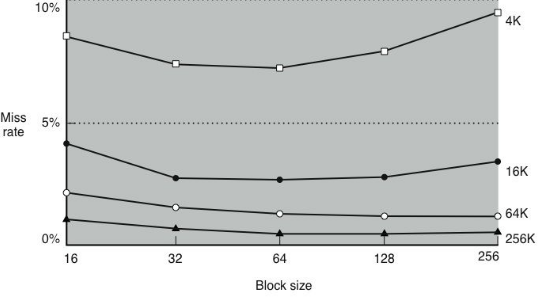
\includegraphics[scale=0.5]{03-Cache/Linee cache.png}
    \caption{Confronto sulla dimensione delle linee du cache.}
\end{figure}

\subsection{Il supporto della RAM}

\dfn{Coerenza della Cache}{
  Una linea in RAM e la corrispondente copia in cache sono sempre identiche. 
}

\cor{Write-Through}{
  Le scritture vengono sempre eseguite sia in cache che in RAM in modo che i dati presenti nelle due memorie siano sempre consistenti tra di loro.
}

\nt{Lo schema Write-Through non offre buone prestazioni perché richiede l'accesso, per ogni scrittura in cache, anche l'accesso alla RAM (il ché consuma molti cicli di clock).}

\cor{Write-Back}{
  Il valore viene modificato solo nella cache. La modifica viene propagata in RAM (o ai livelli successivi di cache) solo se il dato stesso dev essere rimpiazzato da un altro con cui condivide lo stessi tag.
}

\paragraph{}

Si consideri un sistema a 32 bit (e quindi con un bus sulla
scheda madre a 32 bit). Se si suppone che un
accesso alla RAM richieda 15 cicli di clock per leggere una word da
32 bit, per servire un cache miss con linee da 16 byte si impiegheranno 65 cicli di clock:

\begin{itemize}
  \item 1 ciclo di clock per inviare l'indirizzo della linea mancante alla RAM. 
  \item 4 x 15 cicli di clock per leggere l'intera linea. 
  \item 4 x 1 cicli di clock per inviare l'intera linea alla cache.
\end{itemize}

\paragraph{}

Si può cercare di migliorare la situazione: 

\begin{itemize}
  \item Allargando la banda passante della RAM, ossia la quantità di dati che possiamo prelevare dalla RAM con un unico accesso. 
  \item Allargando il bus in modo da poter trasportare in un unico ciclo di clock l'intera linea prelevata dalla RAM.
\end{itemize}

\nt{Aumentare l'ampiezza del bus è costoso e non troppo efficiente. Per cui si sceglie di allargare la banda passante dalla RAM.}

\paragraph{}

\dfn{Memoria Interlacciata (Interleaved Memory)}{
  SI organizza la RAM in banchi in modo da poter leggere o scrivere più word (anziché una sola) in parallelo. Se una linea è formata da $n$ word la linea viene distribuita su $n$ banchi di RAM, ciascuno dei quali memorizza una delle $n$ word della linea. Gli altri $n$ banchi possono essere letti in parallelo estraendo così, in una sola lettura, tutte le word di cui è composta una linea. 
}

\nt{Si risparmia sul tempo necessario a prelevare un'intera linea dalla RAM. Applicando questo schema all'esempio precedente si scende da 65 a 20 cicli di clock.}

\subsection{Cache Set-Associative}

Una caratteristica fondamentale delle cache Direct-Mapped, è che una
determinata linea della RAM viene memorizzata sempre nella stessa
entry della cache. Inoltre più linee di RAM fanno riferimento alla stessa entry
della cache, dato che questa è meno capiente della RAM.

\dfn{Cache Set-Associative a n vie}{
  Una cache Set-Associative a n vie è suddivisa in più insiemi ciascuno formato da n entry (2, 4, 6, 8) e può contenere n linee. Ogni linea della RAM corrisponde a uno e un solo insieme e quella linea può essere memorizzata in una qualsiasi delle n entry dell'insieme. In una cache Set-Associative l'insieme che contiene una linea è stabilito da: (numero della linea in RAM) modulo (numero di insiemi della cache).
}

\nt{Quasi sempre nei computer sono presenti queste cache.}

\begin{figure}[!h]
    \centering
    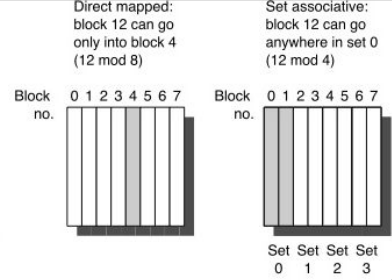
\includegraphics[scale=0.5]{03-Cache/SA.png}
    \caption{Confronto tra Direct-Mapped e Set-Associative.}
\end{figure}

\nt{Nella cache direct mapped, la linea 12 può andare solo nella entry
numero 4. Nella cache set-associativa la linea 12 può andare nella
entry 0 o nella entry 1 dell’insieme zero.}
\paragraph{}
In una cache set-associativa quindi, una volta individuato l’insieme
che può contenere una certa linea, occorre ancora verificare se una
delle entry di quell’insieme contiene la linea indirizzata (il che viene
fatto con una ricerca associativa su tutti gli elementi dell’insieme). Se una linea indirizzata manca, va portata in cache, e inserita in una
qualsiasi entry (è meglio scegliere una entry libera). Se invece tutte le entry dell’insieme sono occupate allora si
sovrascrive una delle linee dell’insieme. Di solito si sacrifica
quella indirizzata meno di recente, con rimpiazzamento LRU (Least Recent Used).

\nt{Le cache Set-Associative sono più sofisticate, quindi richiedono apposito hardware, ma hanno prestazioni maggiori.}

\cor{Cache completamente associativa}{
  In generale, una cache associativa in cui c’è un solo unico grande
insieme, e una linea può essere allocata in una qualsiasi entry della
cache, prende il nome di cache completamente associativa (fully
associative cache).
}

\nt{Sono ancora più efficienti, ma molto più costose (esistono solo a livello teorico).}

\begin{figure}[!h]
    \centering
    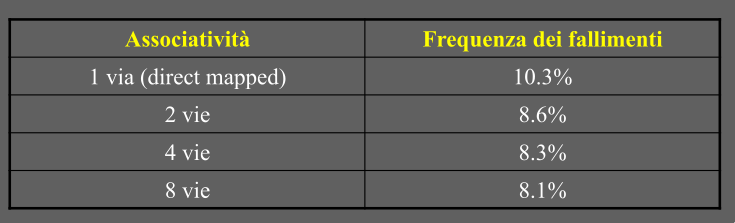
\includegraphics[scale=0.5]{03-Cache/SA2.png}
    \caption{Confronto sul numero di vie.}
\end{figure}

\nt{Servire un cache miss è molto costoso, se si hanno più vie c'è un miglioramento evidente.}

\clm{}{}{
Le cache hanno un effetto positivo in base a quanto:
  \begin{itemize}
    \item Riescono a diminuire il tempo per servire un cache miss. 
    \item Riescono a ridurre il numero di cache miss.
  \end{itemize}
}

\section{Ridurre i Cache Miss}

\subsection{Cache a Più Livelli}

Per ridurre ulteriolmente il numero di cache miss si possono introdurre più livelli di cache. Così facendo si riesce tra l’altro a raggiungere un accettabile trade-
off tra l’avere una cache veloce quanto la CPU (ma costosa, e quindi
piccola) e una cache sufficientemente grande da contenere una buona
parte della RAM (più lenta, ma più economica).

\begin{figure}[!h]
    \centering
    \includegraphics[scale=0.5]{03-Cache/Cache a più livelli.png}
    \caption{I vari livelli di cache, normalmente $L1 \leq L2 \leq L3$.}
\end{figure}

\nt{Nei moderni multi-core, ogni core ha a disposizione L1 ed L2 private,
mentre L3 è condivisa. L1 ed L2 risiedono sullo stesso chip del
processore, mentre L3 può essere:
\begin{itemize}
  \item Sullo stesso chip.
  \item Separato nello stesso package.
  \item Sulla motherboard.
\end{itemize}
}

\paragraph{In un sistema con almeno due livelli di cache:}

\begin{enumerate}
  \item La cache di primo livello deve avere un tempo di accesso simile alla velocità della CPU per non rallentare l'esecuzione in caso di \fancyglitter{cache hit}. 
  \item La cache di secondo livello deve avere una dimensione maggiore della cache di primo livello per ridurre il  numero di \fancyglitter{cache miss} rispetto alla cache di primo livello. 
  \item Lo stesso ragionamento vale per la cache di terzo livello rispetto a quella di secondo. 
\end{enumerate}

\begin{figure}[!h]
    \centering
    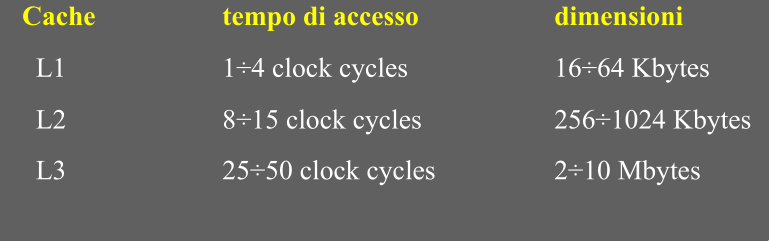
\includegraphics[scale=0.5]{03-Cache/Dati.png}
    \caption{I dati sulle dimensioni sono un po' outdated tbh.}
\end{figure}

\subsection{Ulteriore Riduzione}

Un'altro modo per ridurre il numero di cache miss è quello di rendere l'utilizzo della cache il più efficace possibile, per esempio con una cache Set-Associative, ma anche aumentando le dimensioni delle linee o della cache stessa. 

Normalmente, gli algoritmi sono valutati solo a livello teorico, in
base al numero di operazioni da compiere per risolvere un problema,
rispetto alla “dimensione” del problema. A livello pratico tuttavia, il modo in cui un computer funziona può
influenzare enormemente le effettive prestazioni di un programma. La presenza della cache è uno degli aspetti pratici, nell’esecuzione
dei programmi, che può influenzarne enormemente i tempi di
esecuzione. Un algoritmo che sembra più efficiente di altri a livello teorico,
può in realtà fornire prestazioni peggiori se fatto girare su un sistema
che usa un sistema di cache.
Un esempio è il Radix Sort, un algoritmo di ordinamento che,
per array molto grandi (milioni di elementi), fornisce prestazioni
migliori del Quick Sort in termini del numero di operazioni
richieste per l’ordinamento.

\begin{figure}[!h]
    \centering
    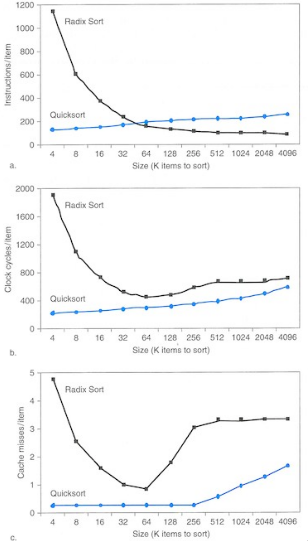
\includegraphics[scale=0.5]{03-Cache/sort.png}
    \caption{Prestazioni di quick sort e radix sort a confronto.}
\end{figure}

\nt{Il radix sort genera più cache miss e quindi a livello pratico è peggiore del quick sort.}

\section{Tecnologie}

\dfn{DIMM}{
  DIMM: Dual Inline Memory Modules. I chip di DRAM sono
normalmente montati su piccole schede contenenti da 4 a 16 DRAM
organizzate in modo da memorizzare i dati in blocchi di 8 bytes
(+ ECC).
}

\dfn{SDRAM}{
  SDRAM: Synchronous DRAM. Sono DRAM dotate di un clock, in
modo da potersi sincronizzare col clock del controller della RAM, e
ottimizzare le prestazioni.
}

\dfn{DDR}{
  DDR: Double Data Rate. Sono SDRAM in cui è
possibile trasferire dati sia sul fronte discendente che su quello
ascendente del clock, in questo modo raddoppiando le prestazioni
rispetto a normali DRAM.
}

\cor{DDR n}{
  DDR2, DDR3, DDR4… L’acronimo DDR indica ormai
comunemente una sequenza di standard, in cui viene man mano
aumentato il clock della DRAM, e quindi la quantità di dati trasferiti
per secondo
}

\nt{Viene anche diminuito il voltaggio di funzionamento, in
modo da diminuire i consumi. DDR=2,5 volt; DDR2= 1,8 volt;
DDR3=1,5 volts; DDR4=1,2 volts.}

\begin{figure}[!h]
    \centering
    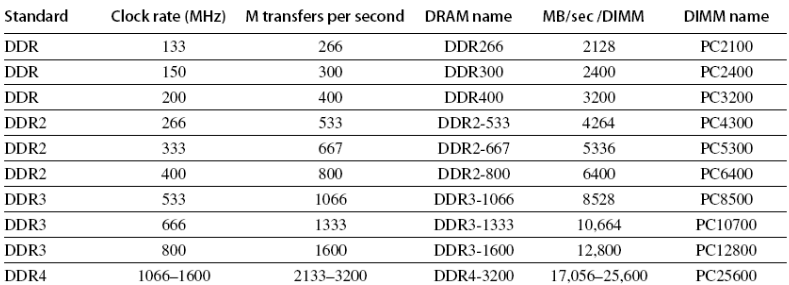
\includegraphics[scale=0.5]{03-Cache/DDR.png}
    \caption{Prestazioni delle DRAM nel 2010.}
\end{figure}

\dfn{GDRAM}{
  GDRAM: Graphics (Synchronous) DRAM. Sono particolari tipi
di DDR (e infatti sono anche denominate GDDR) adatte a gestire le
alte larghezze di banda richieste dai processori grafici:
\begin{itemize}
  \item Trasferiscono più bit in parallelo rispetto alle DRAM. 
  \item Sono saldate sulla GPU per diminuire la dispersione del segnale e aumentare la frequenza di clock.
\end{itemize}

}

\dfn{FLASH Memory}{
  FLASH Memory. Sono particolari tipi di EEPROM (Electronically
Erasable Programmable Read-Only Memory): possono non solo
essere lette, ma anche riscritte. Tuttavia, la riscrittura avviene a
livello di interi blocchi di dati, ossia anche i dati non modificati del
blocco vanno riscritti.
}

\paragraph{Le memorie FLASH sono:}
\begin{itemize}
  \item Statiche, quindi mantengono i dati anche se non alimentate. 
  \item Hanno un numero di cicli di riscrittura limitato a circa 100k per blocco. 
  \item Meno costose delle SDRAM, ma più costose degli Hard Disk. 
  \item In lettura poco più lente delle SDRAM, ma 1000 volte più veloci degli Hard Disk. Ma in scrittura le prestazioni peggiorano molto.
\end{itemize}









